%%
%% ProofForge — AIBT 2026
%% ACM SIGCONF format using acmart document class
%%
\documentclass[sigconf]{acmart}

%% Rights management information
\setcopyright{acmcopyright}
\copyrightyear{2026}
\acmYear{2026}
\acmDOI{XXXXXXX.XXXXXXX}

%% Conference
\acmConference[AIBT 2026]{International Conference on AI and Blockchain Technology}{July 3--5, 2026}{Shanghai, China}
\acmISBN{978-1-4503-XXXX-X/26/07}

%% Packages
\usepackage{booktabs}
\usepackage{listings}
\usepackage{xcolor}
\usepackage{tikz}
\usetikzlibrary{shapes.geometric, arrows.meta, positioning, fit, calc, backgrounds}
\usepackage{enumitem}
\usepackage{tabularx}
\usepackage{array}
\usepackage{makecell}

%% Listings style
\lstdefinelanguage{lean4}{
  keywords={def, namespace, open, import, inductive, structure, deriving, where, if, then, else, let, do, return, match, with, some, none, true, false},
  keywordstyle=\color{blue!70!black}\bfseries,
  ndkeywords={Nat, String, Bool, Unit, Array, IO, Option, Int, UInt32, UInt64},
  ndkeywordstyle=\color{purple!70!black},
  comment=[l]{/-},
  commentstyle=\color{gray!80}\itshape,
  morecomment=[l]{--},
  string=[b]",
  stringstyle=\color{green!60!black},
  sensitive=true,
}

\lstset{
  language=lean4,
  basicstyle=\ttfamily\scriptsize,
  breaklines=true,
  showstringspaces=false,
  numbers=none,
  frame=single,
  framerule=0.4pt,
  rulecolor=\color{gray!50},
  backgroundcolor=\color{gray!5},
  xleftmargin=2pt,
  xrightmargin=2pt,
  aboveskip=4pt,
  belowskip=4pt,
}

\lstdefinestyle{textcode}{
  language={},
  basicstyle=\ttfamily\scriptsize,
  breaklines=true,
  frame=single,
  framerule=0.4pt,
  rulecolor=\color{gray!50},
  backgroundcolor=\color{gray!5},
  keywordstyle=,
  commentstyle=,
  stringstyle=,
}

%% Compact table font
\newcommand{\tsum}{\footnotesize}
\newcommand{\ttab}{\scriptsize}
\setlength{\headheight}{15.5pt}

%% TikZ styles
\tikzset{
  block/.style={
    rectangle, rounded corners=2pt, draw=blue!50!black, fill=blue!8,
    minimum height=7mm, minimum width=22mm, font=\small\sffamily,
    inner sep=4pt, align=center, line width=0.5pt
  },
  coreblock/.style={
    rectangle, rounded corners=2pt, draw=teal!60!black, fill=teal!10,
    minimum height=7mm, minimum width=30mm, font=\small\sffamily,
    inner sep=4pt, align=center, line width=0.5pt
  },
  targetblock/.style={
    rectangle, rounded corners=2pt, draw=orange!70!black, fill=orange!10,
    minimum height=6mm, minimum width=20mm, font=\footnotesize\sffamily,
    inner sep=3pt, align=center, line width=0.5pt
  },
  artifactblock/.style={
    rectangle, rounded corners=2pt, draw=gray!60!black, fill=gray!8,
    minimum height=6mm, minimum width=20mm, font=\footnotesize\sffamily,
    inner sep=3pt, align=center, line width=0.5pt
  },
  gate/.style={
    diamond, draw=red!60!black, fill=red!8, aspect=2,
    minimum height=8mm, font=\footnotesize\sffamily,
    inner sep=2pt, align=center, line width=0.5pt
  },
  arrow/.style={-Stealth, thick, draw=blue!50!black},
  bidir/.style={Stealth-Stealth, thick, draw=gray!60!black, dashed},
  fvarrow/.style={-Stealth, thick, draw=teal!50!black},
}

\begin{document}

%%
%% Title
%%
\title{ProofForge: A Lean-First Multi-Chain Smart Contract\\Compilation Platform with Compile-Time Capability Verification}

%%
%% Authors
%%
\author{DaviRain Su}
\email{davirain.dev@gmail.com}
\affiliation{%
  \institution{Independent Researcher}
  \city{Shanghai}
  \country{China}
}

\renewcommand{\shortauthors}{Su}

%%
%% Abstract
%%
\begin{abstract}
Smart contract development across heterogeneous blockchain platforms (EVM, Solana, NEAR,
Move-based chains, ZK circuits) remains fragmented: each ecosystem demands its own language,
toolchain, and security audit. We present \textbf{ProofForge}, a Lean-first multi-chain smart
contract compilation platform that enables developers to write contract business logic,
state-machine rules, and verification annotations once in Lean~4, then compile to
chain-native artifacts across multiple target families through a single portable
intermediate representation (IR).
The platform's core innovation is a \emph{capability-based routing model}: each target declares
which capabilities it supports, and the compiler rejects unsupported contract intents at
compile time rather than silently changing semantics. We describe the four-layer architecture
(authoring SDK $\to$ ContractSpec $\to$ portable IR $\to$ target backends), the capability
registry with 23 registered capability identifiers across 10 target profiles, and three
P0-signed primary backends---EVM (via Yul/solc), Solana sBPF (direct assembly), and
NEAR/Wasm (via EmitWat). The platform includes executable IR semantics with
\texttt{decide}-checked trace obligations where implemented, ownership checks for
heap-backed locals, and a staged formal verification roadmap (FV-1 through FV-8).
The unified testkit achieves behavior parity and resource budget baselines for the
Counter and ValueVault shared scenarios across all three primary targets. Gate~P0---the
primary-chain completion covenant---is closed as of July~2026.
\end{abstract}

%%
%% CCS Concepts
%%
\begin{CCSXML}
<ccs2012>
 <concept>
  <concept_id>10011007.10011074.10011099</concept_id>
  <concept_desc>Software and its engineering~Compilers</concept_desc>
  <concept_significance>500</concept_significance>
 </concept>
 <concept>
  <concept_id>10011007.10011074.10011111</concept_id>
  <concept_desc>Software and its engineering~Software verification and validation</concept_desc>
  <concept_significance>500</concept_significance>
 </concept>
 <concept>
  <concept_id>10002978.10003029</concept_id>
  <concept_desc>Security and privacy~Distributed systems security</concept_desc>
  <concept_significance>300</concept_significance>
 </concept>
</ccs2012>
\end{CCSXML}

\ccsdesc[500]{Software and its engineering~Compilers}
\ccsdesc[500]{Software and its engineering~Software verification and validation}
\ccsdesc[300]{Security and privacy~Distributed systems security}

\keywords{smart contracts, multi-chain compilation, Lean 4, portable intermediate representation, capability routing, formal verification, EVM, Solana, NEAR, WebAssembly}

%% No teaserfigure — it overlaps title. Pipeline goes to Figure 1 after intro.

\maketitle

%% =====================================================
%% 1. INTRODUCTION
%% =====================================================
\section{Introduction}

The blockchain ecosystem has fragmented into isolated platform silos---Ethereum (EVM), Solana
(sBPF), NEAR (Wasm), Aptos/Sui (Move), and ZK circuit targets---each with its own programming
language, virtual machine, storage model, and toolchain. A contract deployed on Ethereum
cannot run on Solana; a Solana program cannot execute on NEAR. Cross-chain deployment requires
complete rewrites, duplicate security audits, and platform-specific testing, leading to
duplicated effort and inconsistent guarantees.

Existing multi-chain approaches attempt to solve this through either (a) a ``lowest common
denominator'' language that abstracts away platform differences~\cite{reach} or (b) transpilation
between platform-native languages~\cite{solang}. Both approaches have fundamental limitations:
the former cannot express platform-specific features (Solana PDAs, EVM delegate calls, Move
resources), and the latter risks semantic drift during translation. Neither approach integrates
formal verification into the compilation pipeline.

We present \textbf{ProofForge}~\cite{proofforge}, a Lean-first multi-chain smart contract
compilation platform built on three design principles:

\begin{enumerate}[leftmargin=*]
  \item \textbf{Proof-oriented source, multiple targets.} Contract logic,
  state-machine rules, and invariants are written once in Lean~4~\cite{lean4}. The compiler lowers them through a
  portable intermediate representation to chain-native artifacts.
  \item \textbf{Reject, don't silently change semantics.} A capability-based routing model
  ensures that if a contract uses an operation unsupported by the selected target, the compiler
  emits a diagnostic with the specific capability identifier and target identifier---rather than
  producing incorrect code.
  \item \textbf{Verification belongs before codegen.} Executable semantics,
  trace obligations, and future proof obligations are checked in Lean before or alongside
  backend lowering, not retrofitted after deployment.
\end{enumerate}

ProofForge currently supports three P0-signed primary backends: EVM (via Yul and
\texttt{solc}~\cite{yul}), Solana (via direct sBPF assembly to ELF~\cite{solana}), and NEAR (via
EmitWat to Wasm~\cite{near,wasm}). Additional backends for Aleo Leo (ZK~\cite{aleo}),
Cloudflare Workers (off-chain), and Move (Aptos~\cite{move}) are in research or frozen-spike
stages. The platform has closed Gate~P0---the primary-chain completion covenant---meaning all
three primary targets pass behavior parity and resource budget tests for the shared Counter and
ValueVault scenarios. Figure~\ref{fig:pipeline} shows the overall compilation pipeline.
Here, ``P0-signed'' means the repository's production-grade gate for the shared scenario
surface: target-first emission/build, local execution or deployment smoke, artifact/deploy
metadata, capability diagnostics, resource budgets, and green CI evidence. It does not claim
full SDK ecosystem completeness for arbitrary contracts.

\begin{figure*}[t]
  \centering
  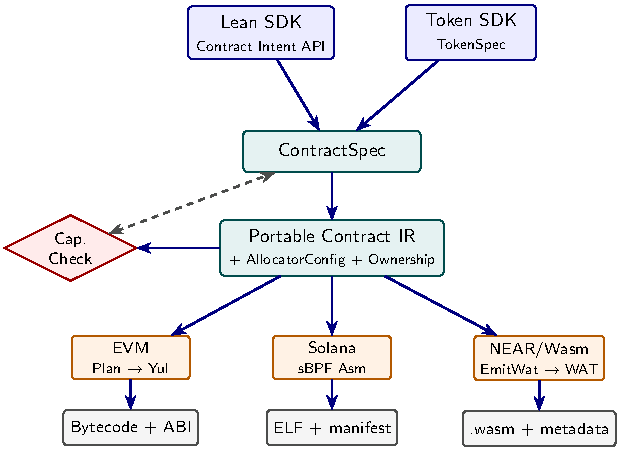
\includegraphics[width=0.85\textwidth]{pipeline-figure}
  \caption{ProofForge compilation pipeline. Lean source lowers through ContractSpec to a
  portable IR, which is routed via capability checks to target-specific backends. Unsupported
  capabilities are rejected before artifact generation.}
  \Description{A vertical pipeline diagram showing the flow from Lean SDK and Token SDK through
  ContractSpec, Portable Contract IR, capability check, and then branching to EVM, Solana,
  and NEAR/Wasm backends, each producing chain-native artifacts.}
  \label{fig:pipeline}
\end{figure*}

This paper makes the following contributions:

\begin{itemize}[leftmargin=*]
  \item A \textbf{portable contract IR} with typed effects, ownership rules, and capability
  annotations that sits between chain-neutral contract logic and target-specific backends
  (\S\ref{sec:arch}).
  \item A \textbf{capability routing model} with 23 registered capability identifiers across 10
  target profiles, enabling compile-time rejection of unsupported operations (\S\ref{sec:cap}).
  \item Three \textbf{P0-signed backends} (EVM/Yul, Solana/sBPF-asm, NEAR/EmitWat)
  with artifact emission, deployment metadata, and validation gates for the shared
  P0 scenario surface
  (\S\ref{sec:backends}).
  \item An \textbf{executable IR semantics} with \texttt{decide}-checked trace obligations and a
  staged formal verification roadmap (\S\ref{sec:fv}).
  \item A \textbf{unified testkit} achieving behavior parity and resource budget baselines for
  shared scenarios across three blockchain target families (\S\ref{sec:eval}).
\end{itemize}

%% =====================================================
%% 2. BACKGROUND
%% =====================================================
\section{Background and Motivation}
\label{sec:bg}

\subsection{The Multi-Chain Problem}

Smart contract platforms differ along multiple dimensions that make cross-chain compilation
non-trivial. Table~\ref{tab:diffs} summarizes the key semantic differences.

\begin{table*}[t]
  \caption{Key semantic differences across blockchain target families.}
  \label{tab:diffs}
  \centering
  \ttab
  \begin{tabularx}{\textwidth}{l X X X X}
    \toprule
    \bfseries Dimension & \bfseries EVM & \bfseries Solana & \bfseries NEAR & \bfseries Move \\
    \midrule
    State model & Global slot storage & Account data & Key-value store & Resources / objects \\
    Execution model & Stack VM & sBPF register VM & Wasm host & Move VM \\
    Cross-contract call & \texttt{CALL}/\texttt{DELEGATECALL} & CPI with account metas & Async promises & Module calls \\
    Identity & \texttt{msg.sender} & Signer accounts & Predecessor account & Transaction sender \\
    Value transfer & \texttt{msg.value} (wei) & SOL via system program & \noindent attached deposit & Module resources \\
    Resource budget & Gas & Compute units (CU) & Gas (Tgas) & Gas \\
    Heap management & None (scratch memory) & Bump allocator & Host-managed & VM-managed \\
    \bottomrule
  \end{tabularx}
\end{table*}

These differences mean a naive ``write once, run everywhere'' approach either (a)~restricts
contracts to the intersection of all platforms, losing platform-specific capabilities, or
(b)~silently maps operations to incorrect semantics, introducing security vulnerabilities. For
example, Solana's Program-Derived Addresses (PDAs) and Cross-Program Invocations (CPI) have no
direct EVM analog, while EVM's \texttt{DELEGATECALL} has no Solana equivalent.

\subsection{Lean 4 as a Contract Language}

Lean~4~\cite{lean4} is a purely functional programming language with dependent types and a
built-in theorem prover. Its key properties make it suitable for smart contract development:
\begin{itemize}[leftmargin=*]
  \item \textbf{Dependent types} enable expressing invariants like ``the sum of balances equals
  the total supply'' at the type level.
  \item \textbf{Proof terms} can be constructed and checked before code generation, ensuring
  that verified properties hold at runtime.
  \item \textbf{LCNF} (Lean Compiler Normal Form) provides a CPS-style intermediate
  representation that ProofForge lowers through EmitYul for EVM targets.
  \item \textbf{Metaprogramming} allows the Contract Intent API to be embedded as a
  domain-specific language within Lean itself.
\end{itemize}

\subsection{Related Work}

\textbf{Reach}~\cite{reach} is the closest precedent: a domain-specific language for writing
multi-chain contracts. However, Reach does not integrate formal proofs, and its semantics are
determined at the language level rather than through a capability model. \textbf{Solang}~\cite{solang}
compiles Solidity to non-EVM targets (Solana, Polkadot) but starts from an EVM-centric source
language and cannot express platform-native patterns. \textbf{Move}~\cite{move} provides
resource-oriented programming for Aptos/Sui but is tied to the Move VM. \textbf{Certora}~\cite{certora}
provides formal verification for EVM contracts but targets a single chain. No existing platform
combines Lean~4's proof capabilities with multi-chain compilation through a capability-routed
portable IR.

%% =====================================================
%% 3. ARCHITECTURE
%% =====================================================
\section{Architecture}
\label{sec:arch}

ProofForge's architecture follows a four-layer model, designed to separate concerns between
contract logic, target routing, and artifact generation.

\subsection{Layer 1: Authoring SDK (Contract Intent API)}

The default SDK surface is the \textbf{Contract Intent API}, a chain-neutral interface that
exposes state declarations, entrypoints, events, caller/value access, checked arithmetic,
assertions, and proofs---without importing any destination-chain module. The API deliberately
does not expose EVM storage slots, Solana account metas, Move resources, or Wasm host ABIs.

For contracts that need chain-specific semantics (e.g., Solana PDA/CPI),
\textbf{Target Extension SDKs} provide explicit chain-native operations. These extensions lower
through capability identifiers and target metadata rather than adding chain-only constructors
to the portable IR (Decision D-027), ensuring the IR remains chain-neutral.

The Contract Intent API also includes a multi-chain \textbf{Token SDK}
(\texttt{TokenSpec}) that routes one token intent to ERC-20 bytecode on EVM or SPL
Token / Token-2022 deployment plans on Solana.

\subsection{Layer 2: ContractSpec}

The \texttt{ContractSpec} is the compiler-owned intermediate representation produced from the
authoring SDK. It captures the contract's declared entrypoints, state, events, and invariants
without any target-specific information. The spec is the input to the portable IR extractor and
the capability resolution phase.

\subsection{Layer 3: Portable Contract IR}
\label{sec:ir}

The portable IR is the central abstraction of the platform. It sits between the chain-neutral
ContractSpec and target-specific backends, expressing chain-independent business logic plus
target-resolved capability effects. The IR is defined in \texttt{ProofForge.IR.Contract} as a
set of Lean~4 inductive types. Figure~\ref{fig:ir-overview} shows the IR module structure and
its relationship to the compilation pipeline.

\begin{figure}[t]
  \centering
  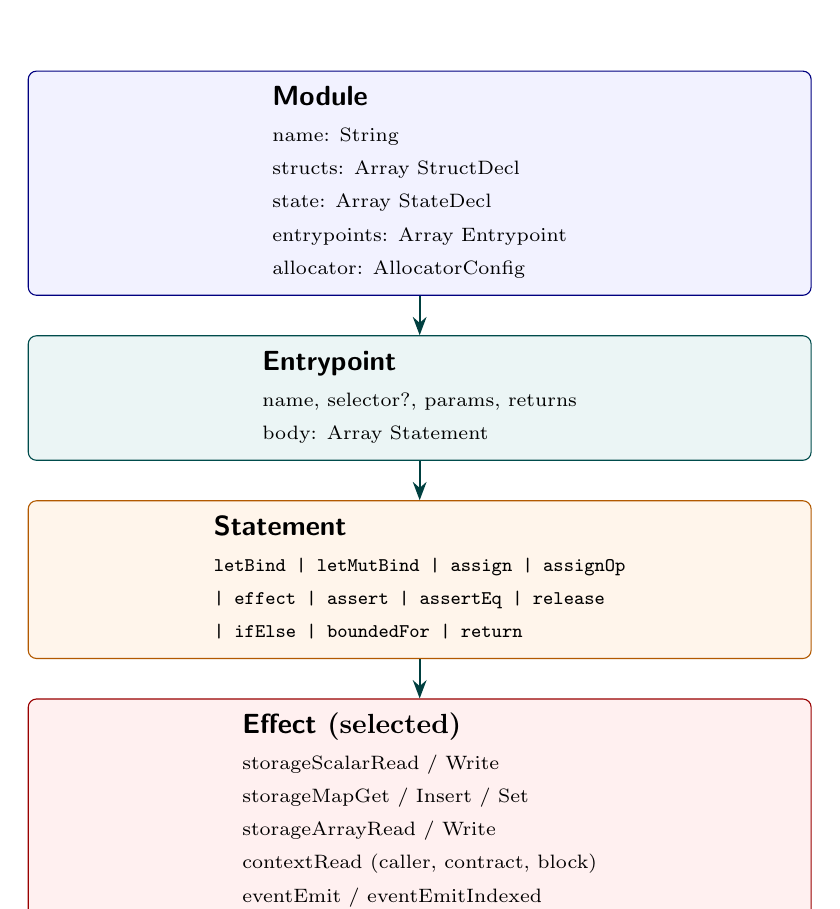
\begin{tikzpicture}[node distance=5mm]
    %% Module structure
    \node[draw=blue!50!black, rounded corners=3pt, fill=blue!5, inner sep=4pt, minimum width=0.82\columnwidth] (mod) {
      \begin{tabular}{l}
        \textbf{\textsf{Module}} \\[1pt]
        \scriptsize name: String \\
        \scriptsize structs: Array StructDecl \\
        \scriptsize state: Array StateDecl \\
        \scriptsize entrypoints: Array Entrypoint \\
        \scriptsize allocator: AllocatorConfig \\
      \end{tabular}
    };

    %% Entrypoint structure
    \node[draw=teal!60!black, rounded corners=3pt, fill=teal!8, inner sep=4pt, minimum width=0.82\columnwidth, below=of mod] (ep) {
      \begin{tabular}{l}
        \textbf{\textsf{Entrypoint}} \\[1pt]
        \scriptsize name, selector?, params, returns \\
        \scriptsize body: Array Statement \\
      \end{tabular}
    };

    %% Statement types
    \node[draw=orange!70!black, rounded corners=3pt, fill=orange!8, inner sep=4pt, minimum width=0.82\columnwidth, below=of ep] (stmt) {
      \begin{tabular}{l}
        \textbf{\textsf{Statement}} \\[1pt]
        \scriptsize \texttt{letBind | letMutBind | assign | assignOp} \\
        \scriptsize \texttt{| effect | assert | assertEq | release} \\
        \scriptsize \texttt{| ifElse | boundedFor | return} \\
      \end{tabular}
    };

    %% Effect types
    \node[draw=red!60!black, rounded corners=3pt, fill=red!6, inner sep=4pt, minimum width=0.82\columnwidth, below=of stmt] (eff) {
      \begin{tabular}{l}
        \textbf{\textsf{Effect} (selected)} \\[1pt]
        \scriptsize storageScalarRead / Write \\
        \scriptsize storageMapGet / Insert / Set \\
        \scriptsize storageArrayRead / Write \\
        \scriptsize contextRead (caller, contract, block) \\
        \scriptsize eventEmit / eventEmitIndexed \\
      \end{tabular}
    };

    %% Arrows
    \draw[fvarrow] (mod) -- (ep);
    \draw[fvarrow] (ep) -- (stmt);
    \draw[fvarrow] (stmt) -- (eff);

  \end{tikzpicture}
  \caption{Portable IR module structure. A Module contains state declarations
  and typed entrypoints. Each entrypoint body is a sequence of statements, which
  may produce typed effects that carry capability identifiers.}
  \Description{A vertical diagram showing Module containing Entrypoints, which contain
  Statements, which may produce Effects.}
  \label{fig:ir-overview}
\end{figure}

Each effect node carries a capability identifier derivable from the effect constructor via the
\texttt{Effect.capability} function. This mapping is the basis for compile-time capability
checking: the target adapter inspects the capabilities used by the IR and rejects the build if
any are unsupported. The key IR types are:

\begin{lstlisting}
inductive ValueType where
  | unit | bool | u32 | u64 | hash
  | fixedArray (element : ValueType) (length : Nat)
  | structType (name : String)

inductive Statement where
  | letBind (name : String) (type : ValueType) (value : Expr)
  | letMutBind (name : String) (type : ValueType) (value : Expr)
  | assign (target value : Expr)
  | assignOp (target : Expr) (op : AssignOp) (value : Expr)
  | effect (effect : Effect)
  | assert (condition : Expr) (message : String)
  | release (name : String)  -- release owned local
  | ifElse (condition : Expr) (thenBody elseBody : Array Statement)
  | boundedFor (indexName : String) (start stopExclusive : Nat) (body : Array Statement)
  | return (value : Expr)

structure Module where
  name : String
  structs : Array StructDecl := #[]
  state : Array StateDecl
  entrypoints : Array Entrypoint
  allocator : AllocatorConfig := defaultAllocator
\end{lstlisting}

The shared scenario Counter contract, expressed as portable IR, demonstrates how one module
lowers to multiple targets without modification:

\begin{lstlisting}
def module : Module := {
  name := "Counter"
  state := #[{ id := "count", kind := .scalar, type := .u64 }]
  entrypoints := #[
    { name := "initialize", returns := .unit,
      body := #[.effect (.storageScalarWrite "count" (.literal (.u64 0)))] },
    { name := "increment", returns := .unit,
      body := #[
        .letBind "n" .u64 (.effect (.storageScalarRead "count")),
        .effect (.storageScalarWrite "count"
          (.add (.local "n") (.literal (.u64 1)))) ] },
    { name := "get", returns := .u64,
      body := #[.return (.effect (.storageScalarRead "count")) ] }
  ]
}
\end{lstlisting}

This same IR module lowers to EVM Yul (with storage slot mapping), Solana sBPF assembly (with
account data read/write), and NEAR WAT (with key-value storage)---without any modification to
the IR itself.

\subsection{Layer 4: Target Backends}

Each target backend is responsible for: (1)~declaring a target profile (supported capabilities,
allocator config, metadata); (2)~lowering accepted IR constructs to target-native code;
(3)~rejecting unsupported constructs with explicit diagnostics; and (4)~emitting artifacts
(bytecode, ELF, Wasm) plus deployment manifests and ABI/IDL metadata. The target registry
(\texttt{ProofForge.Target.Registry}) maintains profiles for each registered target id. The
CLI selects the target via \texttt{-{}-target~<id>}, which activates the corresponding adapter
and capability set.

%% =====================================================
%% 4. CAPABILITY ROUTING
%% =====================================================
\section{Capability-Based Target Routing}
\label{sec:cap}

The capability model is ProofForge's core design principle: \emph{a contract that routes to a
target only uses capabilities that target supports}. Unlike a monolithic IR where all constructs
are available on all targets, ProofForge's IR marks each effect with a capability identifier,
and the target adapter checks support before lowering.

\subsection{Capability Registry}

The canonical capability registry defines 23 core capability identifiers across 13 domains.
The implementation registry currently contains 10 target profiles, including historical
Solana routes retained for compatibility; Table~\ref{tab:capreg} shows the support matrix
for the primary and representative active targets.

\begin{table*}[t]
  \caption{Core capability registry (selected). Y = supported, P = partial/spike, N = not supported.}
  \label{tab:capreg}
  \centering
  \ttab
  \begin{tabular}{l c c c c c}
    \toprule
    \bfseries Capability ID & \bfseries EVM & \bfseries NEAR & \bfseries Solana & \bfseries Psy & \bfseries CF W. \\
    \midrule
    \texttt{storage.scalar}        & Y & Y & Y & Y & Y \\
    \texttt{storage.map}           & Y & Y & P & P & Y \\
    \texttt{storage.array}        & P & N & Y & P & P \\
    \texttt{caller.sender}         & Y & Y & Y & P & Y \\
    \texttt{value.native}          & Y & Y & Y & P & N \\
    \texttt{events.emit}           & Y & Y & Y & Y & Y \\
    \texttt{crosscall.invoke}      & Y & N & N & P & Y \\
    \texttt{crosscall.cpi}         & N & N & Y & N & N \\
    \texttt{storage.pda}           & N & N & Y & N & N \\
    \texttt{crypto.hash}           & Y & Y & Y & Y & Y \\
    \texttt{assertions.check}      & Y & Y & Y & P & Y \\
    \texttt{control.conditional}  & P & N & Y & Y & Y \\
    \texttt{control.bounded\_loop} & N & N & P & P & Y \\
    \texttt{zk.circuit}            & N & N & N & Y & N \\
    \texttt{runtime.allocator}    & N & Y & Y & P & N \\
    \bottomrule
  \end{tabular}
\end{table*}

\subsection{Capability Resolution}

When the compiler receives a \texttt{-{}-target} flag, it performs the resolution sequence
shown in Figure~\ref{fig:cap-flow}.

\begin{figure}[t]
  \centering
  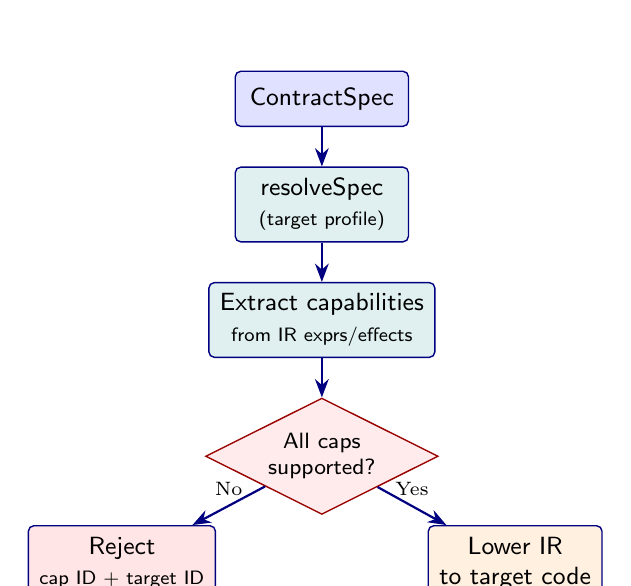
\begin{tikzpicture}[node distance=5mm]
    \node[block, fill=blue!12] (spec) {ContractSpec};
    \node[block, fill=teal!12, below=of spec] (resolve) {resolveSpec\\\scriptsize (target profile)};
    \node[block, fill=teal!12, below=of resolve] (extract) {Extract capabilities\\\scriptsize from IR exprs/effects};
    \node[gate, below=of extract] (check) {All caps\\supported?};
    \node[block, fill=red!10, below left=5mm and 6mm of check] (reject) {Reject\\\scriptsize cap ID + target ID};
    \node[block, fill=orange!12, below right=5mm and 6mm of check] (lower) {Lower IR\\to target code};

    \draw[arrow] (spec) -- (resolve);
    \draw[arrow] (resolve) -- (extract);
    \draw[arrow] (extract) -- (check);
    \draw[arrow] (check) -- node[font=\scriptsize, above] {No} (reject);
    \draw[arrow] (check) -- node[font=\scriptsize, above] {Yes} (lower);
  \end{tikzpicture}
  \caption{Capability resolution flow. The target adapter resolves the contract spec,
  extracts required capabilities from the IR, and checks them against the target profile.
  Unsupported capabilities produce a diagnostic; only fully-supported contracts proceed to lowering.}
  \Description{A flowchart: ContractSpec feeds into resolveSpec, then capability extraction,
  then a decision diamond. If all capabilities are supported, the IR is lowered to target code;
  otherwise, a rejection diagnostic is emitted.}
  \label{fig:cap-flow}
\end{figure}

\subsection{Ownership and Allocator Model}

The IR includes an ownership system for heap-backed locals (the \texttt{release} statement).
The checker in \texttt{IR/Ownership.lean} rejects use-after-release and double-release
patterns. Each target configures its allocator via \texttt{AllocatorConfig}; see
Table~\ref{tab:alloc}.

\begin{table}[t]
  \caption{Allocator configuration per target.}
  \label{tab:alloc}
  \centering
  \ttab
  \begin{tabularx}{\columnwidth}{l l X l}
    \toprule
    \bfseries Target & \bfseries Strategy & \bfseries Region & \bfseries Release \\
    \midrule
    EVM & Bump & Call-scratch memory & None (rejected) \\
    Solana & Bump & Heap at \texttt{0x300000000} & Noop \\
    NEAR & Host & Wasm linear memory & Noop \\
    \bottomrule
  \end{tabularx}
\end{table}

The ownership checker ensures that the three different lowerings of \texttt{release}
(EVM rejects it, Solana lowers to a no-op, NEAR lowers to \texttt{memory.free}) are safe
only if the IR-level discipline is proven (FV-3 target).

%% =====================================================
%% 5. BACKENDS
%% =====================================================
\section{Backend Implementations}
\label{sec:backends}

\subsection{EVM Backend (Baseline)}

The EVM backend is the most mature target. The pipeline:

\begin{lstlisting}[style=textcode]
Lean contract source
  -> Lean frontend / LCNF
  -> EmitYul (LCNF -> Yul AST)
  -> Yul source
  -> solc --strict-assembly
  -> EVM runtime bytecode
  -> Foundry smoke tests
\end{lstlisting}

For portable IR contracts, the EVM backend introduces a \textbf{semantic plan layer} between
the IR and Yul generation (RFC~0004). The plan defines \texttt{ExprPlan}, \texttt{StmtPlan},
\texttt{EntrypointPlan}, \texttt{EventPlan}, \texttt{CrosscallPlan}, and \texttt{MetadataPlan},
which are validated and type-inferred before Yul generation. This separation ensures that the
Yul output is type-correct and that checked arithmetic semantics (trap on overflow) are
enforced at the plan level.

The EVM SDK (\texttt{ProofForge.Evm}) provides extern declarations for EVM opcodes such as
\texttt{calldataload}, \texttt{sstore}, \texttt{sload}, \texttt{caller}, and \texttt{keccak256}.
EmitYul recognizes these externs and lowers them directly to EVM instructions. Typed
storage helpers provide compile-time slot assignment and mapping slot computation.

Validation gates include: 58 diagnostic cases, 99 IR coverage entries, 19 IR smoke tests,
Foundry runtime smoke tests, and Anvil deploy tests~\cite{foundry}.

\subsection{Solana sBPF Assembly Backend}

The Solana backend generates sBPF assembly directly from the portable IR, bypassing
intermediate languages like Zig or Rust (Decision D-026). The pipeline:

\begin{lstlisting}[style=textcode]
portable IR
  -> sBPF assembly (.s)
  -> sbpf toolchain (assemble + link)
  -> ELF (.so) program binary
  -> Mollusk / Surfpool / Pinocchio tests
\end{lstlisting}

The backend defines Solana-specific constructs in the Solana SDK layer:
\begin{itemize}[leftmargin=*,nosep]
  \item account metas and signer policies;
  \item PDA bindings with seeds and bump values;
  \item CPI calls with account metas and signer seeds;
  \item sysvar, memory, crypto-hash, and compute-budget actions.
\end{itemize}

These Solana-specific constructs are gated by \texttt{crosscall.cpi} and \texttt{storage.pda}
capabilities (D-027) and never appear in the portable IR itself---they live in the Solana
backend and SDK layer.

Validation includes Pinocchio~\cite{pinocchio} live dual-deploy equivalence tests across five
scenarios (System transfer/create\_account, SPL Token transfer/ops/authority), all passing with
\texttt{5 passed, 0 skipped, 0 failed}. The ELF compatibility blocker was resolved by forwarding
\texttt{-{}-solana-sbpf-arch~v0}, producing loader-compatible v0 ELFs.

\subsection{NEAR/Wasm Backend (EmitWat)}

The NEAR backend uses EmitWat, which lowers portable IR to a Wasm AST and then to WAT
(WebAssembly Text Format) text, compiled to \texttt{.wasm} via \texttt{wat2wasm}~\cite{wasm}.
This approach mirrors the EVM's portable-IR-to-Yul pattern:

\begin{lstlisting}[style=textcode]
portable IR
  -> EmitWat (Wasm AST construction)
  -> WAT text
  -> wat2wasm
  -> .wasm binary
  -> offline host execution / NEAR deployment
\end{lstlisting}

EmitWat avoids Rust \texttt{near-sdk-rs} macro coupling (D-031) and the Lean-runtime-to-Wasm
port that blocked prior approaches. Because the portable IR already abstracts over Lean
objects, EmitWat needs no Lean runtime port, object-model boxing, or garbage collection.

The NEAR backend includes target-first \texttt{check}, \texttt{emit}, and \texttt{build}
commands. It writes artifact and deploy manifests, validates WAT/Wasm hashes,
ABI entrypoints, and capabilities, and executes the generated Counter WAT through
an offline host.

\subsection{Research and Frozen Backends}

Additional backends exist in research or frozen-spike stages:
\begin{itemize}[leftmargin=*,nosep]
  \item \textbf{Psy/DPN} and \textbf{Aleo Leo}~\cite{aleo};
  \item \textbf{Cloudflare Workers};
  \item \textbf{Move/Aptos}~\cite{move} and \textbf{CosmWasm}~\cite{cosmwasm}.
\end{itemize}
These paths are useful architecture probes, but they are outside the P0 production-grade claim.

%% =====================================================
%% 6. FORMAL VERIFICATION
%% =====================================================
\section{Formal Verification}
\label{sec:fv}

ProofForge is Lean-first, but most current assurance comes from executable semantics,
trace obligations, tests, and golden files rather than complete metatheory. The formal
verification roadmap (FV-1 through FV-8) progressively turns test-validated invariants into
machine-checked theorems. The intended model is compile-time proof checking and no proof
transport to chains: Lean proofs are not verified on-chain.

\subsection{Existing Formal Anchors}

Three verification anchors are already implemented on \texttt{main}; see Table~\ref{tab:fv}.

\begin{table*}[t]
  \caption{Existing formal verification anchors.}
  \label{tab:fv}
  \centering
  \ttab
  \begin{tabularx}{\textwidth}{l X}
    \toprule
    \bfseries Anchor & \bfseries What it provides \\
    \midrule
    IR Semantics \scriptsize(\texttt{IR/Semantics.lean}) & Executable trace interpreter for the covered scalar, aggregate, storage, control-flow, and event slices; \texttt{decide}-checked \\
    \addlinespace
    Ownership Rules \scriptsize(\texttt{IR/Ownership.lean}) & Static \texttt{release}/owned-local checker; FV-3 will prove semantic no-use-after-release and no-double-release soundness \\
    \addlinespace
    Trace Obligations \scriptsize(\texttt{Backend/*/Refinement.lean}) & \texttt{decide}-checked obligations: EVM/Yul covers Counter, ValueVault, and focused probe traces; NEAR/WAT currently anchors the Counter IR trace/export surface \\
    \bottomrule
  \end{tabularx}
\end{table*}

\subsection{Verification Targets (Priority Order)}

Figure~\ref{fig:fv-roadmap} shows the staged FV roadmap and its dependency structure.

\begin{figure}[t]
  \centering
  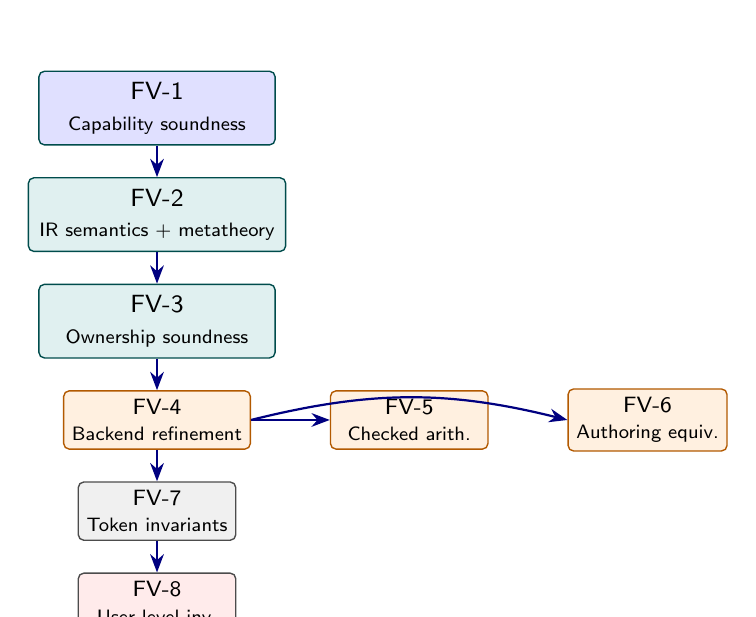
\begin{tikzpicture}[node distance=4mm and 6mm]
    \node[coreblock, fill=blue!12] (fv1) {FV-1\\\scriptsize Capability soundness};
    \node[coreblock, fill=teal!12, below=of fv1] (fv2) {FV-2\\\scriptsize IR semantics + metatheory};
    \node[coreblock, fill=teal!12, below=of fv2] (fv3) {FV-3\\\scriptsize Ownership soundness};
    \node[targetblock, fill=orange!12, below=of fv3] (fv4) {FV-4\\\scriptsize Backend refinement};
    \node[targetblock, fill=orange!12, right=10mm of fv4] (fv5) {FV-5\\\scriptsize Checked arith.};
    \node[targetblock, fill=orange!12, right=10mm of fv5] (fv6) {FV-6\\\scriptsize Authoring equiv.};
    \node[artifactblock, fill=gray!12, below=of fv4] (fv7) {FV-7\\\scriptsize Token invariants};
    \node[artifactblock, fill=red!8, below=of fv7] (fv8) {FV-8\\\scriptsize User-level inv.};

    \draw[arrow] (fv1) -- (fv2);
    \draw[arrow] (fv2) -- (fv3);
    \draw[arrow] (fv3) -- (fv4);
    \draw[arrow] (fv4.east) -- (fv5.west);
    \draw[arrow] (fv4.east) to[bend left=14] (fv6.west);
    \draw[arrow] (fv4) -- (fv7);
    \draw[arrow] (fv7) -- (fv8);
  \end{tikzpicture}
  \caption{Formal verification roadmap. FV-1 (capability soundness) and FV-2 (IR semantics)
  are foundational. FV-3 depends on FV-2. FV-4 (backend refinement) builds on FV-3.
  FV-5/FV-6 stabilize target surfaces. FV-7/FV-8 are product-level proofs.}
  \Description{A dependency diagram showing FV-1 at top, flowing down through FV-2, FV-3,
  FV-4, FV-7, and FV-8. FV-5 and FV-6 branch from FV-4 at the same level.}
  \label{fig:fv-roadmap}
\end{figure}

\textbf{FV-1 (Capability Routing Soundness):} Prove that a successful
\texttt{resolveSpec} result only contains capabilities supported by the target profile.
Also prove rejection completeness: if the spec references an unsupported capability,
resolution returns an error. These are structural inductions over arrays---no semantics needed.

\textbf{FV-2 (IR Semantics):} Extend \texttt{IR/Semantics.lean} from the scalar subset toward
the full checked IR surface. State and prove: determinism (one trace per input/state), progress
and preservation for the typed subset, and bounded termination for \texttt{boundedFor} with
static bounds. Keep the semantics executable (\texttt{decide}-friendly) so CI checks stay cheap.

\textbf{FV-3 (Ownership/Release Soundness):} Once FV-2 gives release-aware semantics, prove
that programs accepted by the ownership checker never evaluate a released local and never
release twice. This justifies target-specific \texttt{release} lowering choices: allocator
frees in EmitWat, rejection on EVM/Psy, and no-op treatment in TS.

\textbf{FV-4 (Backend Refinement):} Replicate the \texttt{TraceObligation} pattern per backend
against the shared scenario (Counter first, ValueVault second). Each backend earns
``Experimental $\to$ Supported'' only with the scenario differential gate and at least the
export/trace obligation theorem.

\textbf{FV-5--FV-8:} Checked arithmetic semantics per target (FV-5), authoring-surface
equivalence for \texttt{.learn} and \texttt{contract\_source} (FV-6), token plan invariants
(FV-7), and user-level contract invariants (FV-8)---the long-term differentiator that lets
contract authors prove properties like $\textit{balance} = \textit{deposits} - \textit{releases} + \textit{fees}$
before codegen.

%% =====================================================
%% 7. EVALUATION
%% =====================================================
\section{Evaluation}
\label{sec:eval}

\subsection{Shared Scenarios}

ProofForge defines two shared scenarios for cross-target validation:
\textbf{Counter} (a minimal stateful contract with \texttt{initialize}, \texttt{increment},
and \texttt{get}, testing scalar storage, arithmetic, and return values) and
\textbf{ValueVault} (a complex contract with deposits, releases, fees, and balance invariants,
testing events, access control, and aggregate state).

\subsection{Behavior Parity}

The unified testkit (RFC~0007) executes the shared scenarios across all three primary targets
and verifies trace parity. Table~\ref{tab:parity} summarizes the results.

\begin{table}[t]
  \caption{Testkit behavior parity results (Gate G0). All three primary targets pass
  Counter, ValueVault (11 calls), and unsupported-capability diagnostic tests.}
  \label{tab:parity}
  \centering
  \ttab
  \begin{tabular}{lccc}
    \toprule
    \bfseries Scenario & \bfseries EVM & \bfseries Solana & \bfseries NEAR \\
    \midrule
    Counter trace        & \checkmark & \checkmark & \checkmark \\
    ValueVault (11 calls) & \checkmark & \checkmark & \checkmark \\
    Unsupported cap. diag. & \checkmark & \checkmark & \checkmark \\
    \bottomrule
  \end{tabular}
\end{table}

\subsection{Resource Budgets}

Per D-040, Tier-0 parity requires comparing behavior \emph{and} resource budgets. The testkit
scenarios pin budget baselines with tolerance bands for EVM gas, Solana compute units (CU), and
NEAR gas (Tgas). Table~\ref{tab:validation} summarizes the validation coverage per target.
Rows marked ``---'' are target-specific gates rather than missing P0 evidence; the shared rows
apply to all three primary targets.

\begin{table*}[t]
  \caption{Dedicated and shared validation gate coverage per primary target.}
  \label{tab:validation}
  \centering
  \ttab
  \begin{tabularx}{\textwidth}{X c c c}
    \toprule
    \bfseries Gate & \bfseries EVM & \bfseries Solana sBPF & \bfseries NEAR/Wasm \\
    \midrule
    Shared scenario behavior parity & \checkmark & \checkmark & \checkmark \\
    Resource budget baselines       & \checkmark & \checkmark & \checkmark \\
    Diagnostic cases              & 58 & --- & --- \\
    IR coverage entries            & 99 & --- & --- \\
    IR smoke tests                 & 19 & --- & --- \\
    Foundry runtime smoke          & \checkmark & --- & --- \\
    Anvil deploy smoke             & \checkmark & --- & --- \\
    Mollusk unit tests             & --- & \checkmark & --- \\
    Surfpool/Web3.js live smokes   & --- & \checkmark & --- \\
    Pinocchio equivalence gates     & --- & 5 scenarios & --- \\
    Offline host smoke             & --- & --- & \checkmark \\
    Formal trace obligations       & \texttt{decide}-checked & --- & \texttt{decide}-checked \\
    Artifact / deploy metadata     & \checkmark & \checkmark & \checkmark \\
    Capability diagnostics         & \checkmark & \checkmark & \checkmark \\
    \bottomrule
  \end{tabularx}
\end{table*}

\subsection{Gate P0 Closure}

Gate~P0---the primary-chain completion covenant (D-045)---was closed on July~4, 2026, at commit
\texttt{466b320}, after GitHub CI run \texttt{28677055773} completed successfully. The closing
run validated all three primary targets including behavior parity, resource budgets,
capability diagnostics, Foundry/Anvil gates, Mollusk/Surfpool gates, offline host execution,
artifact/deploy metadata, and formal trace obligations.

\subsection{Comparison with Existing Approaches}

Table~\ref{tab:compare} compares ProofForge with the two closest multi-chain platforms.

\begin{table*}[t]
  \caption{Comparison with multi-chain contract platforms.}
  \label{tab:compare}
  \centering
  \ttab
  \begin{tabularx}{\textwidth}{l X X X}
    \toprule
    \bfseries Feature & \bfseries ProofForge & \bfseries Reach & \bfseries Solang \\
    \midrule
    Source language        & Lean 4 & Reach DSL & Solidity \\
    Formal proofs          & Lean anchors + roadmap & Linear temporal logic & No \\
    Capability model       & 23 IDs, 10 profiles & Network-specific & EVM-centric \\
    Compile-time reject    & Capability + target ID & Partial & No \\
    Targets                & EVM + Solana + NEAR & EVM + Algorand & Solana + Polkadot \\
    Portable IR            & Yes (typed effects) & Partial & No \\
    Ownership system       & IR-level checker & No & No \\
    Trace obligations      & \texttt{decide}-checked & No & No \\
    \bottomrule
  \end{tabularx}
\end{table*}

%% =====================================================
%% 8. DISCUSSION
%% =====================================================
\section{Discussion}
\label{sec:disc}

\subsection{Design Decisions}

The platform's architecture is guided by 45 settled design decisions (D-001 through D-045), each
documented with rationale and date. Key decisions include: \textbf{D-027} (CPI/PDA effects stay
in a Solana-specific layer, not the portable IR); \textbf{D-028} (user contracts target a
chain-neutral Contract Intent API; the selected target resolves intents into capability plans);
\textbf{D-031} (EmitWat is the canonical Wasm-family backend); and \textbf{D-045} (the three
priority chains must be completed to P0 production-grade quality before any additional chain
advances beyond docs-only research).

\subsection{Limitations}

Current limitations include: the portable IR expression set is a contract-relevant subset of
Lean/LCNF, not full Lean preservation---higher-order functions, closures, and unbounded loops
are restricted or rejected on most targets. Formal verification is in early stages: FV-1 through
FV-3 are planned but not yet implemented; only FV-2 (executable IR semantics) and FV-4 (trace
obligations) have \texttt{decide}-checked theorems. The EVM backend has the most mature validation
surface; Solana and NEAR have fewer dedicated gates. The CLI is mid-migration from legacy flags
to \texttt{proof-forge build|emit|check -{}-target}; legacy aliases remain for compatibility.

%% =====================================================
%% 9. CONCLUSION
%% =====================================================
\section{Conclusion and Future Work}
\label{sec:concl}

ProofForge demonstrates that a Lean-first, capability-routed architecture can produce P0-grade
smart contract artifacts across heterogeneous blockchain platforms without silently changing
semantics. The platform's core promise---\emph{one proof-oriented contract source, multiple
chain-native artifacts, unsupported operations rejected at compile time}---is validated by
the closure of Gate~P0, with behavior parity and resource budgets confirmed across EVM,
Solana sBPF, and NEAR/Wasm.

The staged formal verification roadmap (FV-1 through FV-8) provides a clear path from the current
test-validated invariants toward machine-checked theorems, starting with capability routing
soundness (FV-1) and IR semantics metatheory (FV-2), culminating in user-level contract invariant
proofs (FV-8)---the long-term differentiator that lets contract authors prove properties like
$\textit{balance} = \textit{deposits} - \textit{releases} + \textit{fees}$ before codegen.

Future work follows the tiered target portfolio (D-034): \textbf{Tier-1}: advance CosmWasm
and Move/Aptos from frozen spikes to M3/M4 after CLI migration completes.
\textbf{Tier-2}: sourcegen targets (Stellar Soroban, Starknet Cairo, TON TVM, Cardano
Plutus/Aiken, Tezos Michelson/LIGO) after two Tier-1 targets reach Experimental.
\textbf{Policy family}: Bitcoin Script/Miniscript, Bitcoin Cash CashScript, Zcash Shielded,
and Kaspa Toccata as spending-policy generators with a separate policy IR.
\textbf{Cloud platform}: hosted target-matrix builds, artifact registry, testnet deployment,
and verification reports.

%% =====================================================
%% ACKNOWLEDGMENTS
%% =====================================================
\begin{acks}
The ProofForge project builds on the Lean~4 theorem prover~\cite{lean4}, the Foundry
development toolkit~\cite{foundry}, the Solana sBPF toolchain~\cite{solana}, and the
NEAR/Wasm ecosystem~\cite{near}. The design was shaped by 45 settled design decisions reviewed
through a structured RFC process.
\end{acks}

%% =====================================================
%% BIBLIOGRAPHY
%% =====================================================
\bibliographystyle{ACM-Reference-Format}
\bibliography{references}

\end{document}
